\chapter{Software development}\label{chp:6}

\minitoc

\clearpage


In this Chapter, we present the design and the implementation of the procedure developed to detect spatio-temporal anomalies described in Chapters \ref{chp:4} and \ref{chp:5}.

%is generic and could handle any substance in any region. 

The implementation was done in two steps. First, for a selected pollutant during a selected period in a selected geographical area, an R script implements the preprocessing of raw data as well as the precomputation of change-point detection in concentration data as described in Chapter \ref{chp:4} and the spatial clustering of measuring stations as described in Chapter \ref{chp:5}. This script can handle the concentration in surface waters of any substance in any region in France. This preprocessing step is described in Section \ref{chp:6:1}, together with the format of the produced output file.

The file produced in the first step is then fed to an Rshiny application, described in Section \ref{chp:6:2}. This application is intended for the ANSES experts in order to analyse pollutant concentration data in surface waters, therefore the interface and user manual are written in French. 

So far, the application can handle Prosulfocarb concentration data only, however it can very easily be extended to other substances in future developments. Three options are available for the user, implemented as three tabs in the main menu. The Home tab, presented in section \ref{chp:6:2:1}, provides an overview of the available information on the substance under consideration (here the Prosulfocarb), as well as basic visualization of the input data. The Detection tab allows the user to perform the anomaly detection procedure described in Chapter \ref{chp:5}. The corresponding implementation is described in Section \ref{chp:6:2:2}. The third tab allows accessing the user manual of the application. This document, intended for users that do not necessarily have a strong mathematical background, is available in Appendix \ref{app:chap6:2}. 

%All the procedure developped to detect spatio-temporal anomalies derived from Chapter \ref{chp:4} and \ref{chp:5} was implemented in an \texttt{Rshiny} application. This application is intended for the ANSES experts to assist them analyzing concentration data. 

%Once a preprocessing is performed on the data of a substance, it can be loaded into the application. When the application starts, three tabs are available: the \textbf{Home tab} to give a overview of the susbtance informations; the \textbf{Detection tab} where the whole procedure of Chapter \ref{chp:5} is implemented; the \textbf{Explanatory note tab} this gives direction on how to use the application. This dociment is intended for people that don't necessary have mathematical background. It explains the events triggered by possible actions in the application.     

%In this Chapter, we present how the application is designed. The presentation follows the tab order in the application. In Section \ref{chp:6:1}, we present the overview tab. We describe the elements composing the Detection tab in Section \ref{chp:6:2}. The explanatory notice is available in \ref{app:chap6:2}. This document is written in french as it is intended for the experts of the agency.  

\section{Data preprocessing and precomputation}\label{chp:6:1}

The raw data to be processed are the three following files that the user has to extract from public databases:
\begin{itemize}
\item[-] A table of the concentration measurements in a given geographical area and during a given time period (in the case of surface waters substances, such tables can be extracted from NAIADE\footnote{see \cite{Naiade2}} database in .csv file format).
\item[-] A table of the station locations (.csv file format extracted from NAIADE database) in Lambert 93 Coordinates Reference System (CRS).
\item[-] For each administrative region (‘département’ in French) in the geographical region of interest, a file providing the coordinates and direction of the hydrographic segments (shapefile format, extracted from the BDTOPO\footnote{see \cite{BDTOPO}} database)
\end{itemize}
An \texttt{R} script was developed to preprocess these data and precompute time-segmentation and spatial clustering. The data preprocessing steps consist of: 
\begin{itemize}
\item[-] The construction of the station graph, according to the method described in Section \ref{subsection:graph:construct}. Its vertices are the stations and its edges indicate a connexion between two stations through the hydrographic network. The edge weights are the length of the shortest existing path of water linking two stations. The graph is stored as a \texttt{igraph} object \citep{igraph}. 
\item[-] The construction of a table for measured concentrations, storing the sampling date, the measurement, a boolean indicating if this value corresponds to a quantified value, the station ID and the LOQ value. All values are converted to $\mu$g/L. The table containing the daily maximum values time series presented in Section \ref{subsection:data:collection} is constructed from this table.
\item[-] The construction of a regional shapefile merging all ``département'' shapefiles, converted to Lambert 93 CRS.
\end{itemize}

For the precomputation step, the change-point detection method proposed in Chapter \ref{chp:4} is implemented for a Weibull distribution. The cost function evaluation and the PELT algorithm are coded with \texttt{Rcpp} for a faster execution, while CROPS algorithm is coded in \texttt{R}.
 
%The following computations are performed:
The following quantities are calculated:
\begin{itemize}
\item[-] The change-point detection in the daily maximal concentration signal in the geographical area of interest. The CROPS algorithm is trained for a penalty range $[\beta_{min},\beta_{max}]$ defined in Section \ref{chp:5:4:1}. The significant penalties selected by CROPS and the associated segmentation results are stored in a list.
%, for the penalty range $[\beta_{min},\beta_{max}]$ defined in Section \ref{sec:time_pattern}. The sequence of penalties and the associated segmentation results computed by the CROPS algorithm are stored.
\item[-] The connected components of the station graph, identified using the available \texttt{components} function in the \texttt{igraph} package.
%are identified using  and algorithm coded in the  \citep{Hopcroft1973}. 
\item[-] The spatial clustering of the station graph is performed using the clustering methods presented in Algorithm \ref{algo:dyn}. We did not use the elbow heuristic to select a unique number of clusters because we wanted to offer the experts the opportunity to explore different values. This is why several clustering results are stored, with their respective number of clusters ranging between a minimal and maximal value. The heuristic used to determine the minimal and maximal number of clusters is presented in Appendix \ref{app:chap6:1}.  
\end{itemize}

The output file of this preprocessing and precomputation procedure is a \texttt{.Rdata} file containing: 
\begin{itemize}
\item[-] The detailed table containing all concentration measures for all stations.
%The table with all concentration measurement information built in the preprocessing step.
\item[-] The table with all daily maximum measurement information built in the preprocessing step.
\item[-] A list with all temporal segmentation results and details obtained by CROPS (parameter values, cost, penalty values etc...).
\item[-] A table with all station coordinates in WGS84 CRS and with all clustering membership results and connected component labels. 
\item[-] A table with all hydrographic segment coordinates in WGS84. 
\item[-] A table with the geographical area border coordinates in WGS84.
\item[-] A table with the border coordinates of the hydro ecoregions in WGS84.
\end{itemize}

\begin{figure}[htbp]
  \centering
  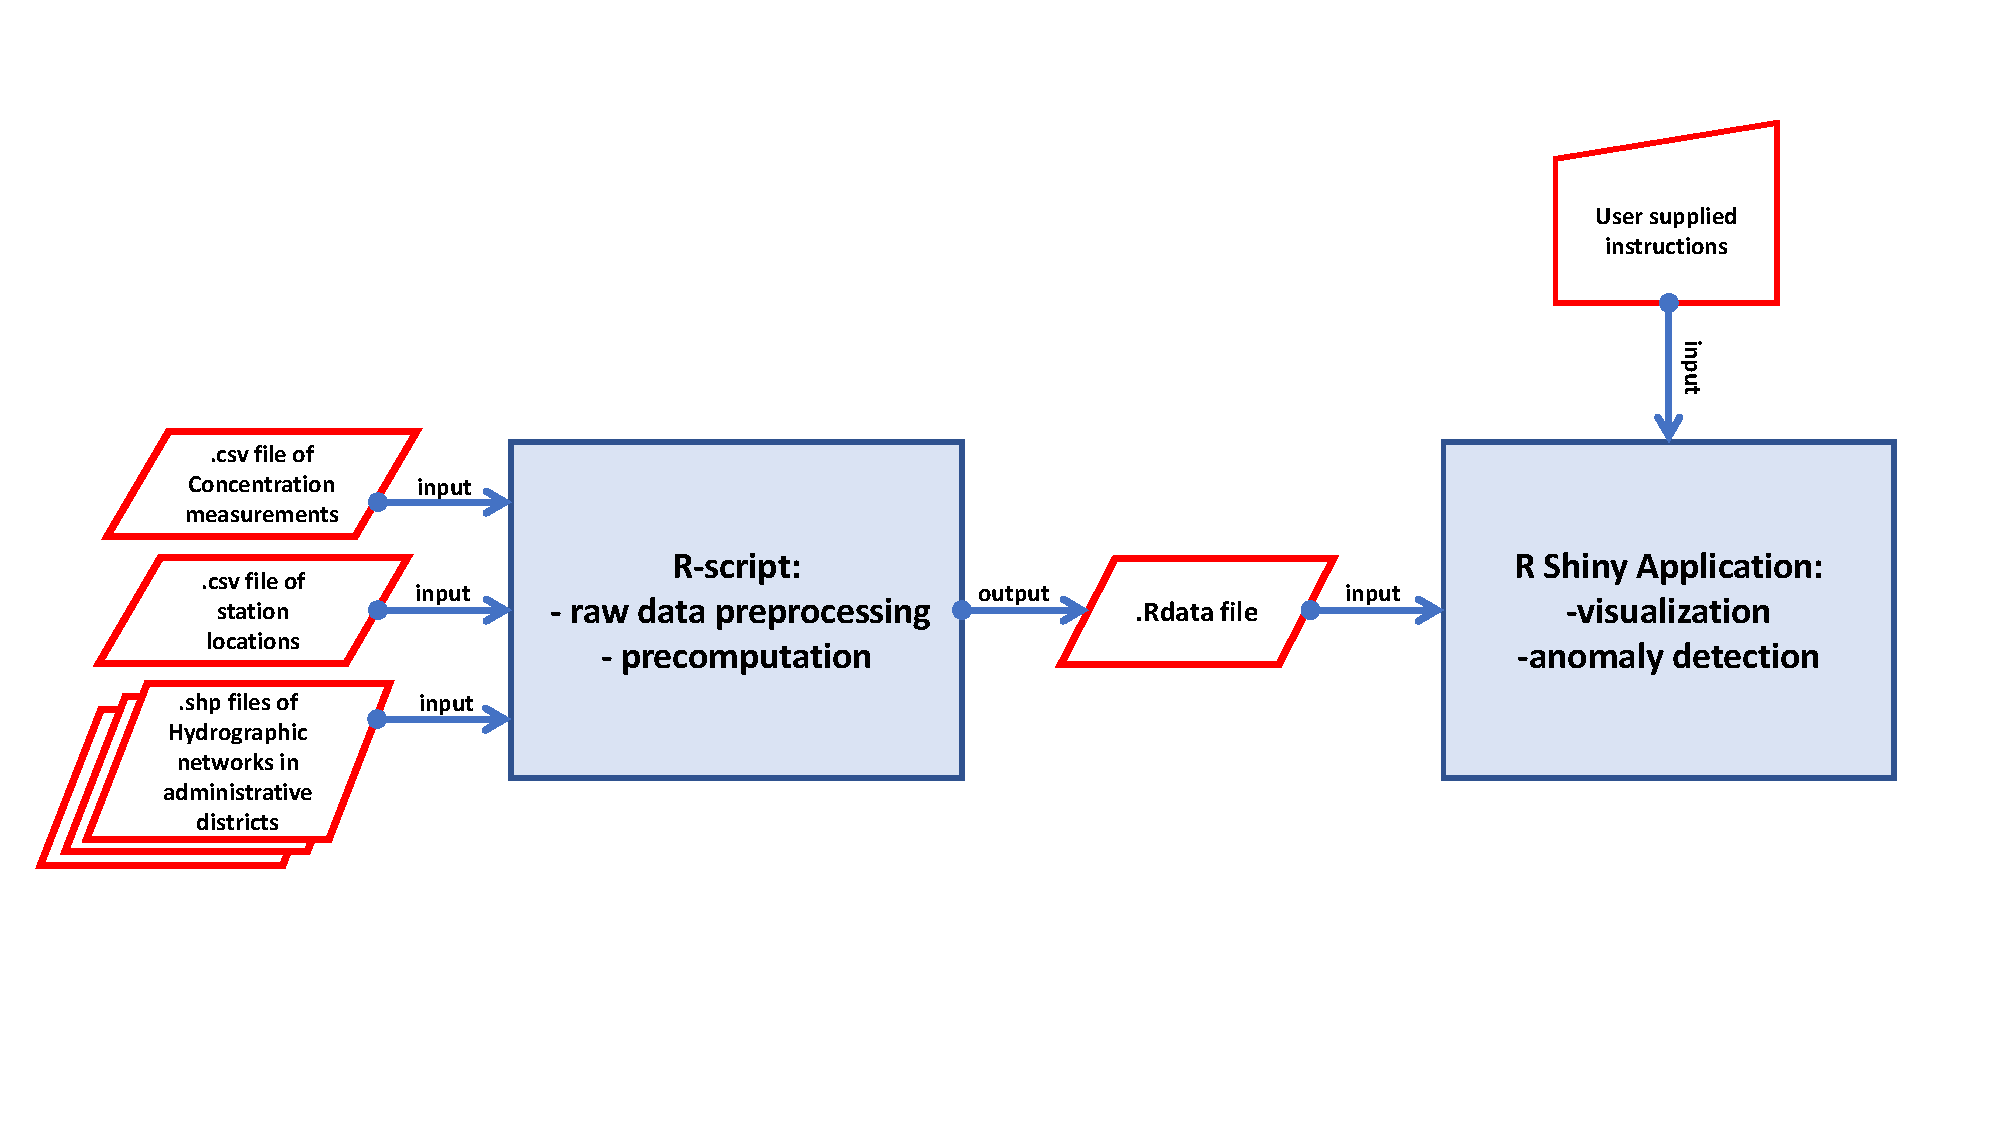
\includegraphics[angle = 90,scale = 0.65]{figs/Chap6/organigramme.pdf}
  \caption{Flowchart summarising the organisation between the preprocessing, precomputation and application steps.}
  \label{fig:orga}
\end{figure}

\section{Rshiny application}\label{chp:6:2}

As mentioned in the introduction, this application aims at visualizing the preprocessed data (subsection \ref{chp:6:2:1}) as well as the results of the anomaly detection procedure described in Chapter \ref{chp:5} (Section \ref{chp:6:2:2}). When the application is started, the \texttt{.Rdata} file generated by the preprocessing step in Section \ref{chp:6:1} from the raw concentration and geographic datasets is automatically uploaded. According to Figure \ref{fig:orga}, this \texttt{.Rdata} file will be referred as the input file in the rest of this section. 

\subsection{Basic visualisation}\label{chp:6:2:1}

%In order to make a quick presentation of the loaded concentration dataset, we display three different elements in this tab.  
  
%The first element is text information where the following precisions are given: 

In this part, which is accessible through the ``Home'' tab, the user can visualize across three panels information contained in the input file.
%from the input file generated in section \ref{chp:6:1} from the raw concentration and geographic datasets across three panels. 

In the first panel, the following basic information is provided:
\begin{itemize}
\item The name of the substance corresponding to the input file uploaded.
\item The dates corresponding the time span in the input data.
\item The geographical area corresponding to the input file uploaded.
\item The total number of measurements collected over the times period.
\item The number of active stations over the time period.
\item The percentage of quantified concentration results among these measurements. 
\item The number of days where at least one sample was recorded. This number is also the number of of daily maximum concentrations. 
\item The percentage of quantified daily maximum concentrations.
\end{itemize}

The second panel (Figure \ref{fig:Imapp1}) displays the plot of the daily maximum concentrations in the geographical area of interest, which allows the experts to visualize the temporal trends and seasonality at a glance, before having any segmentation information that could influence their interpretation.

\begin{figure}[htbp]
  \centering
  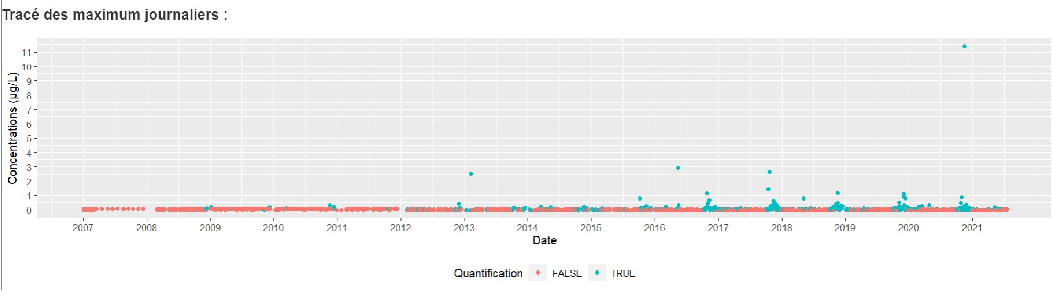
\includegraphics[]{figs/Chap6/Im_app1.pdf}
  \caption{Global temporal presentation.}
  \label{fig:Imapp1}
\end{figure}

The third panel (Figure \ref{fig:Imapp2}) displays the map of the active stations during the period, together with the river network in the area. Based on the preprocessing in section \ref{chp:6:1}, the stations are coloured according to the hydrographic graph connected component they belong to. 

\begin{figure}[htbp]
  \centering
  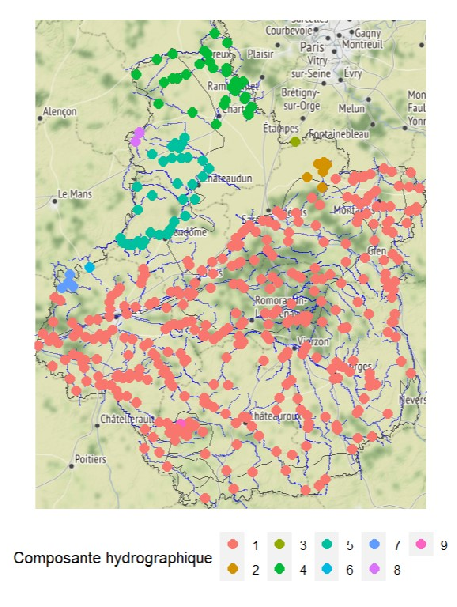
\includegraphics{figs/Chap6/Im_app2.pdf}
  \caption{Global geographical presentation.}
  \label{fig:Imapp2}
\end{figure}

\subsection{Anomaly detection}\label{chp:6:2:2}

This part is accessible to the user through the "Detection” tab. We recall that the anomaly detection procedure described in Chapter \ref{chp:5} consists in three steps, which are a detection of temporal change-points, a spatial clustering of the stations and a procedure for anomaly detection on a given time segment. The results of the first two steps are precomputed and stored in the input file (see Section \ref{chp:6:1}), whereas the third step is performed interactively in the application

\subsubsection{Visualisation of temporal segmentation results}\label{chp:6:2:temp}

%The temporal detection is spread across two information boxes. The first box contains the segmentation performed on the daily maximum time series. Several elements are made available to the user: 
 
The temporal segmentation results are spread across two panels. The first one displays time segmentations performed on the daily maximum time series assuming a Weibull distribution model. Several elements are made available to the user:
\begin{itemize}
\item The plot of the different segmentations cost against their number of change points is displayed, together with a slider allowing to choose a penalty value (see Figure \ref{fig:Imapp3}). For the selected penalty value, the corresponding segmentation is highlighted in red. The red lines on the graph are the two-part linear model obtained using the elbow method Algorithm \ref{chp:3:algoelbow}. The vertical black line indicates the optimal number of change-points detected by CROPS as the abscissa of the elbow position location. The application is initialized on the penalty value corresponding to this optimal number of change-points, however the user may select a non optimal segmentation, which we did on purpose in the Figures. 
\begin{figure}[htbp]
  \centering
  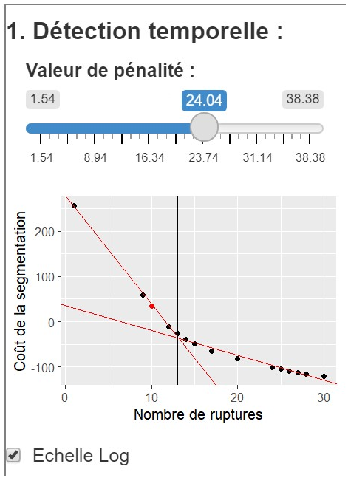
\includegraphics[]{figs/Chap6/Im_appbis3.pdf}
  \caption{Penalty choice and corresponding segmentation information.}
  \label{fig:Imapp3}
\end{figure}
\item A plot of the segmentation of the daily maximum concentration signal (see Figure \ref{fig:Imapp4}). This plot is interactive: it is automatically updated when the user moves the cursor to change the penalty value, and it is also allows the mouse-click selection of a segment in the signal. In this case, it is highlighted in black (see Figure \ref{fig:Imapp4} for an illustration). To better distinguish quantified low concentration values from values under the quantification threshold (which are censored to the current LOQ value), we added the possibility to plot the time series in logarithmic scale to obtain a better visualization. In Figure \ref{fig:Imapp4} concentrations are plotted in logarithmic scale.
\begin{figure}[htbp]
  \centering
  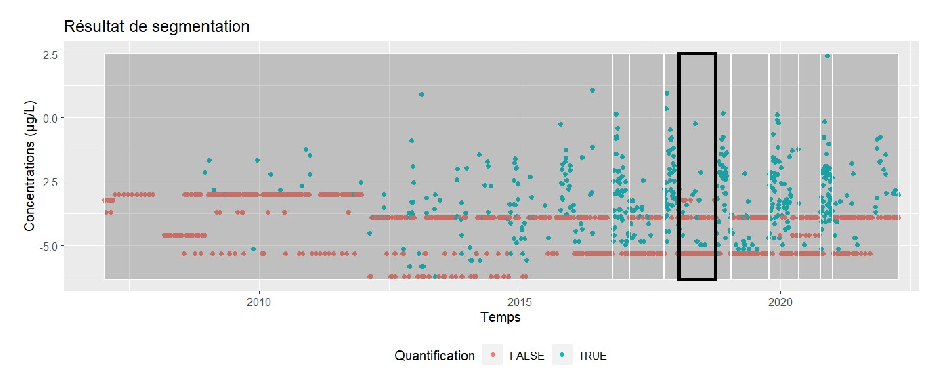
\includegraphics[]{figs/Chap6/Im_appbis4.pdf}
  \caption{Plot of the resulting segmentation.}
  \label{fig:Imapp4}
\end{figure}     
\end{itemize}  

%Several segmentation results of the daily maximum time series are computed with the CROPS algorithm. For each segmentation, we have its corresponding penalty value. A curser to select the penalty value is displayed alongside with a graph of the different segmentations cost against their number of change points (see Figure \ref{fig:Imapp3}). For a selected penalty value in Figure \ref{fig:Imapp3}, the corresponding segmentation is highlighted in red in Figure \ref{fig:Imapp3}. The red lines are the bipartite linear models obtained using the elbow method Algorithm \ref{chp:3:algoelbow}. This provides the indication of what would be the optimal number of change-points. The application starts on the penalty value assoociated to the segmentation which cost is located on the elbow position. We selected a non optimal segmentation on purpose in the figures. 
%Once the penalty value is set, the resulting segmentation on the daily maximum concentration signal is displayed as in Figure \ref{fig:Imapp4}. This element is reactive to the penalty value and update according to the penalty value. It is also possible to select a segment in the signal. In this case, it is highlighted in black. It is the case in Figure \ref{fig:Imapp4}. Lots of concentration values are under the quantification threshold. If some high concentration values occured in the signal, it can be complicated to distinguish low values of concentration. Hence, we added the possibility to plot the time series in logarithmic scale to obtain a better visualization. The concentrations in Figure \ref{fig:Imapp4} are plotted in logarithmic scale.  
%The goodness of fit of the model on the data belonging to the segment selected in Figure \ref{fig:Imapp4} is assessed by comparing the parametric cumulative distribution function to the empirical one. The plot is illustrated in Figure \ref{fig:Imapp5}, vertical black lines are drawned at the LOQ values. The empircal cdf is drawned in blue and the one obtained with the parametric model is drawned in red. The quality of the fit seems satisfactory which conforts the idea that the Weibull law provide a good model for concentration data. 
%The last information is a seasonnal plot. When a segment is selected, we provide a comparison of the violin plot of this segment with similar time periods on the previous and following years. For instance in Figure \ref{fig:Imapp4}, the selected segment spans from the 22nd of January to the 5th of October of the year 2018. We represented the violin plot of the daily maximum concentrations from the 22nd of January to the 5th of October of each year available in Figure \ref{fig:Imapp5}. The violin plot of the selected segment is highlighted in red. Note that the violin plots adapt to whether the logarithmic scale was chosen or not in the previous information box.

A second panel is available for the user, whose content is dependent on the segment selected in the first panel. In this second panel, information specific of the selected segment is displayed:
\begin{itemize}
\item The dates corresponding to the segment temporal limits, the number of daily maximum concentration values inside the segment; the percentage of quantified concentration measurements within the segment; the number of active stations within the segment timespan as well as the minimum, mean, median and maximum values of daily maximum concentrations. 
\item A plot displaying the parametric cumulative distribution function and the empirical one, for visual comparison (see Figure \ref{fig:Imapp5} left). On this plot, vertical black lines are located at the LOQ values. The empirical cdf is coloured in blue and the one obtained with the parametric model is coloured in red. This plot aims at providing a first visual evaluation of the relevance of the parametric distribution used to model the data on the selected segment (a Weibull distribution in the current implementation).  The illustrative example in Figure \ref{fig:Imapp5} confirms the choice of the Weibull distribution as a relevant model for Prosulfocarb concentration data in surface waters.
\item A seasonal plot, providing a comparison of the data violin plot in the currently selected time segment with those computed for the same time periods on the previous and following years. For instance, in Figure \ref{fig:Imapp5}-right, the selected segment spans from the 22nd of January to the 5th of October of the year 2018. We represented the violin plot of the daily maximum concentrations from the 22nd of January to the 5th of October of each year available. The violin plot of the selected segment is highlighted in red. Note that the violin plots adapt to whether the logarithmic scale was chosen or not in the previous panel.
\end{itemize}  

%The following informations are given in the form of text: the dates that define the segment temporal boarders; the number of daily maximum concentration values inside the segment; the quantification percentage of the segment; the number of active stations inside the temporal period defined by the segment; the minimum, the mean, the median and the maximum values of daily maximum concentrations inside the segment.

\begin{figure}[htbp]
  \centering
  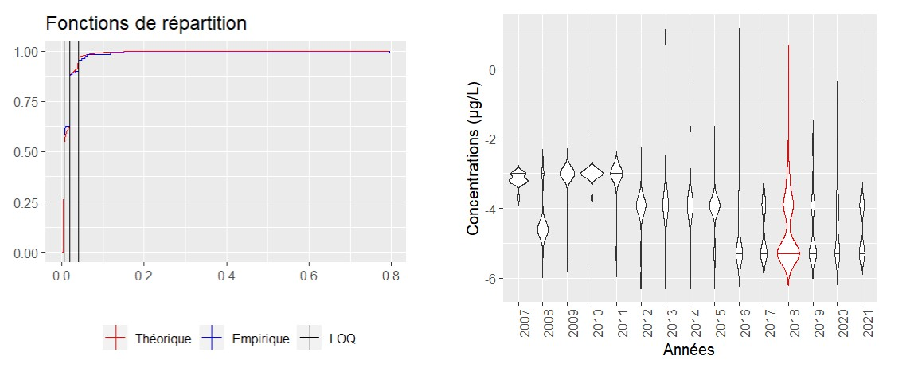
\includegraphics[]{figs/Chap6/Im_appbis5.pdf}
  \caption{Informations on the selected segment.}
  \label{fig:Imapp5}
\end{figure}

These two panel encompass the whole temporal detection procedure. The user selected segment (see Figure \ref{fig:Imapp4}) determines not only the information in the second panel but also all the information that will be presented in the spatial clustering and anomaly detection steps presented in next section.

%This two boxes encompasses the whole temporal detection procedure. The selection of the segment in Figure \ref{fig:Imapp4} determines not only the information in the second box but also all the informations that are presented in the spatial clustering and anomaly detection steps.

\subsubsection{Spatial clustering and anomaly detection}\label{chp:6:2:spat}

%Just as the temporal segmentation, the spatial clustering and the anomaly detection steps are condensed into two information boxes. The first one is a box with a map and several other elements. 

As stated previously, the information provided to the user in this part of the application is dependent of the temporal segment selected in the temporal segmentation panel (see section \ref{chp:6:2:temp}). The spatial clustering and the anomaly detection steps are covered by two additional panels. 

The first one displays a map of the geographical area under consideration and a drop-down menu (see Figure \ref{fig:Imapp}) allowing to choose the information to be displayed on the map. Four different options are available in the menu:
\begin{itemize}
\item "Active station": the stations are plotted with two different colors if they collected a sample during the segment time span or not.
\item "Hydrographic component": the stations are plotted and colored according to which station graph connected component they belong to; note that this information is already available in the "Home tab" but it was repeated here for the user convenience.
\item "Spatial clustering":  the stations are plotted and coloured according to which cluster they belong to (see Figure \ref{fig:Imapp6}).
\item "Pareto front values": stations are plotted and coloured according to their Pareto front level (see Figure \ref{fig:Imapp7}). 
\end{itemize}
%A drop-down menu, illustrated in Figure \ref{fig:Imapp}, is present to choose the information to display on the map. As stated previously, the information is dependant of the temporal segment selected in Section \ref{chp:6:2:temp}. The user can opt for four different options: the information of activity of a station, the stations are colored differently if they made a sample or not during the segment time period; the information of the station graph components, stations are colored according to the component they belong to in the graph of stations; the cluster information, stations are colored according to which cluster they belong to (see Figure \ref{fig:Imapp6}); the pareto front information, stations are colored according to their Pareto front level (see Figure \ref{fig:Imapp7}). The map of the graph component is redundant with the Home tab information but it was still implemented in this box as well to avoid changing tab to get that information. The graph clustering is obtained using the clustering methods presented in Algorithm \ref{algo:dyn}.  
   
\begin{figure}[htbp]
  \centering
  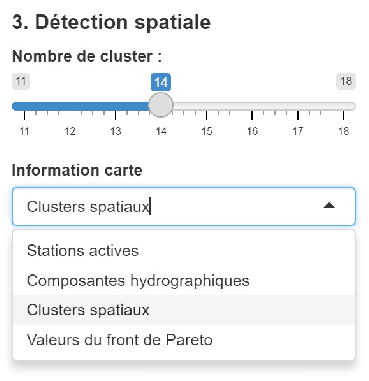
\includegraphics[]{figs/Chap6/Im_appbis.pdf}
  \caption{Drop down menu with curser selecting the number of clusters in the spatial clustering}
  \label{fig:Imapp}
\end{figure}   
   
When "Spatial clustering" or "Pareto front values" are selected, it is necessary to select the desired number of clusters. This number can be selected with a cursor located on the left of the map (not shown in the Figures). The map updates automatically with the selected number of clusters. 
% (see Figure \ref{fig:Imapp6} and \ref{fig:Imapp7})

\begin{figure}[htbp]
  \centering
  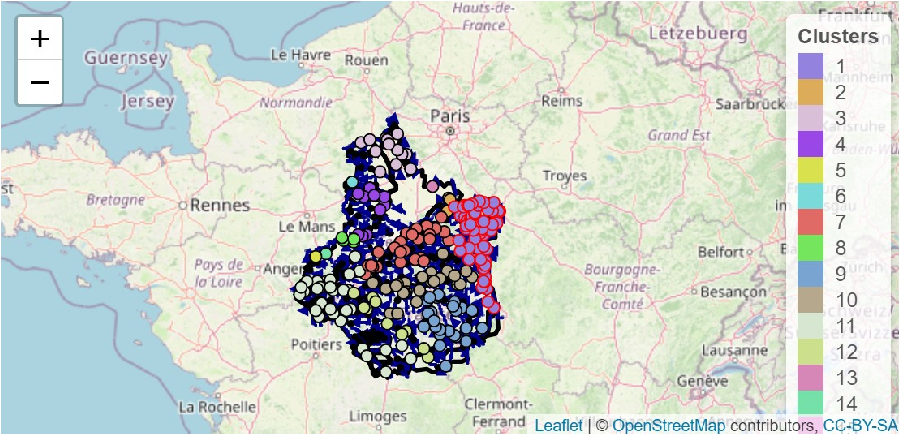
\includegraphics[]{figs/Chap6/Im_appbis6.pdf}
  \caption{Map displaying the clusters. The clustering selected is composed of 14 clusters.}
  \label{fig:Imapp6}
\end{figure}

For "Spatial clustering", the information displayed was computed during the preprocessing step and stored in the input file of the application.   

\begin{figure}[htbp]
  \centering
  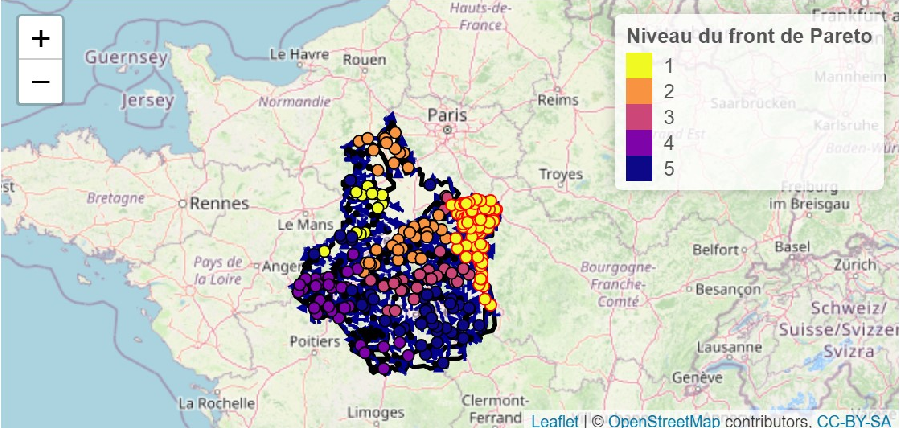
\includegraphics[]{figs/Chap6/Im_appbis7.pdf}
  \caption{Map displaying the Pareto front values of each cluster.}
  \label{fig:Imapp7}
\end{figure}

For "Pareto front values", the Pareto level values are computed and refreshed upon each change in the number of cluster using the \texttt{Rpref} package. The \texttt{Rpref} package implements the multi-criteria optimization using the skyline algorithm \citep{914855}. Additionally, a cluster selection feature is implemented: upon selection of a station, the cluster in which the station is located is highlighted in red as in Figure \ref{fig:Imapp7}. 
%The computations are performed in the application using the . 
%Once the information is set on either the clustering information or the Pareto front levels, it is dependant on the number of cluster information. Several clustering results were imported in the application with their respective number of clusters ranging between two values. The heuristic we use to determine the minimal and maximal values of clusters in the clustering is presented in Appendix \ref{app:chap6:1}. This number can be selected with a curser located on the left in Figure \ref{fig:Imapp6} and \ref{fig:Imapp7}. The map update automatically with the number of clusters information.  


%Additionally, there is a cluster selection feature when selecting on a station. The cluster in which the station is located is highlighted in red as in Figure \ref{fig:Imapp7}. The last box of the tab is dependant of this choice. 

The last panel is dependent on all choices made in the previous panels. It is composed of three windows:   
\begin{itemize}
%The station concentration window: once a station has been selected, this window displays the samples it made during the time period of the selected segment. An illustration is provided in 
%The clusters Pareto plot window:  defined in Section \ref{section:anomaly} .  
\item A Pareto plot where clusters are plotted according to the criteria described in Chapter \ref{chp:5} (see Figure \ref{fig:Imapp8}). The selected cluster in the map is also highlighted in red in the plot.
\begin{figure}[htbp]
 \centering
 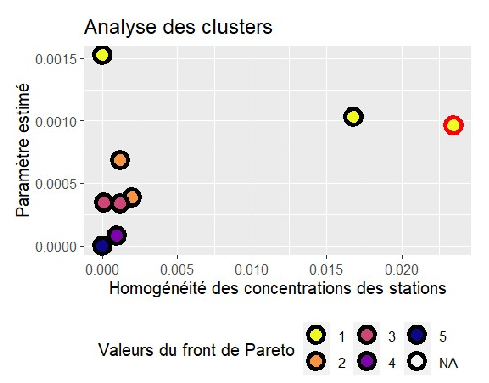
\includegraphics[]{figs/Chap6/Im_appbis8.pdf}
 \caption{Plot of the Pareto front.}
 \label{fig:Imapp8}
\end{figure}
\item Additionnal text information is provided on all measurements in the selected cluster (see Figure \ref{fig:Imapp8}), such as:
\begin{itemize}
\item The total number of measurements collected.
\item The percentage of quantified concentration results among these measurements.
\item The number of active stations in the cluster.
\item The minimum, the mean, the median and the maximum of concentrations.
\item The different LOQ values present in the measurements (the most frequent one being indicated).
\item The station ID with the highest quantification rate and its associated number of measurements and the quantification rate information.
\end{itemize} 
\item A station measurement plot (see Figure \ref{fig:Imapp9}): once a station has been selected in the map, this plot displays its measurements during the selected time segment. 
\begin{figure}[htbp]
 \centering
 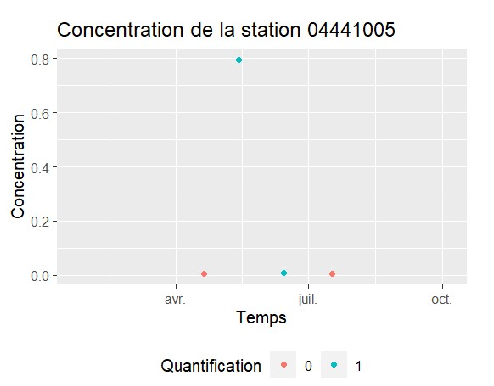
\includegraphics[]{figs/Chap6/Im_appbis9.pdf}
 \caption{Selected station sample values during the selected temporal segment.}
 \label{fig:Imapp9}
\end{figure}
\end{itemize}



%are provided on all samples made by the stations belonging to the selected cluster in the last window such as:  
%made in that cluster in the time period selected; 
%the percentage of quantification of these samples; 
%the number of stations composing the cluster; the minimum, the mean, the median and the maximum of concentration values in the cluster; the LOQ values present in that cluster with the information of the most frequent LOQ; the ID of the station that has the highest quantification rate with its associated percentage of quantification rate and the number of samples that were performed. The LOQ values of a cluster provide an overview of the equipment quality that is installed on the stations.    
